\chapter{Walidacja i wizualizacja}
\label{chap:walidacja}
Utworzenie działającej architektury MoE nie rozstrzyga jeszcze, czy wybór neuronów na podstawie domen SAE przynosi korzyść jakościową lub obliczeniową. W tym celu potrzebna jest walidacja -- zarówno utworzonych ekspertów jak i modelu MoE. Badanie jakości samodzielnych ekspertów bez routera jak i gotowego MoE objęło ocenę modelowania tekstu oraz benchmark składający się z kilku zadań. W niniejszym rozdziale omówiono protokoły tych ocen, wyniki oraz ograniczenia ich interpretacji.

\section{Protokół walidacji i miary jakości}
\label{sec:protokol_walidacji}
Ocenę modelowania tekstu przeprowadzono na zamrożonym zbiorze końcowym obejmującym po $90$ tekstów z każdej domeny oraz $100$ tekstów ogólnych. Były to dane oddzielone od zbioru uczącego, ale pochodzące ze źródeł wykorzystanych w potoku przygotowania domen. Porównano model bazowy, pojedynczych ekspertów, MoE oraz kontrolne przycięcia oparte na maskach losowych i wielkości wag. Mierzono ujemną logarytmiczną wiarygodność kolejnych tokenów, z pominięciem paddingu, oraz jej eksponentę -- perplexity (PPL). Miara ta opisuje, jak dobrze model przewiduje obserwowane tokeny na podstawie ich kontekstu: im większe prawdopodobieństwa im przypisuje, tym niższe są NLL i PPL. Porównanie PPL wymaga tego samego tekstu, tokenizatora i sposobu wyznaczania ocenianych tokenów. Użyto partii po cztery teksty i maksymalnej długości $128$ tokenów. Taki test odpowiada przede wszystkim na pytanie, ile jakości modelowania języka zachowuje rozwiązanie po modyfikacji. \newline
Wspólną miarą dla wszystkich zadań była średnia ujemna logarytmiczna wiarygodność odpowiedzi referencyjnej (ang. \textit{negative log-likelihood}, NLL). Dla przykładu $i$, zawierającego prompt $x_i$ i odpowiedź $y_i$ o długości $L_i$, obliczano:
\[
\operatorname{NLL}_i=-\frac{1}{L_i}\sum_{t=1}^{L_i}
\log p(y_{i,t}\mid x_i,y_{i,<t}),
\qquad
\Delta_i=\operatorname{NLL}_i^{\mathrm{model}}-\operatorname{NLL}_i^{\mathrm{base}}.
\]
Model otrzymuje w tej procedurze poprzednie tokeny poprawnej odpowiedzi (ang. \textit{teacher forcing}); oceniane są wyłącznie tokeny odpowiedzi, bez promptu. Indeks $\mathrm{model}$ oznacza oceniany model dziedzinowy lub MoE, a dodatnia różnica wskazuje pogorszenie względem modelu bazowego. Wyniki ocenianego wariantu i bazy parowano według identyfikatora zadania, a przedziały ufności $95\%$ dla średniej różnicy wyznaczano metodą bootstrapu na poziomie przykładów, z $2000$ replikami. Modele oceniono z partiami po osiem przykładów i limitem $1024$ tokenów.

\subsection{Walidacja modeli dziedzinowych}
\label{subsec:protokol_ekspertow}
Każdy samodzielny model dziedzinowy -- z przyciętym MLP warstwy $9$ oceniono na $100$ przykładach jego własnej domeny. Model bazowy oceniono na wszystkich $600$ przykładach, tworząc kompletne pary baza--właściwy ekspert. Wykorzystany w walidacji zbiór testowy został złożony z kilku źródeł, jak najbardziej zbliżonych do dziedzin wybranych ekspertów. \newline
Prawo, biomedycynę i politykę reprezentowały pytania z testu \textit{MMLU} \cite{hendrycks_2021_measuring_massive_multitask}. Sport oceniano na zadaniu \texttt{sports\_understanding} z BIG-bench \cite{srivastava_2022_beyond_imitation_game}, a Python na zadaniach MBPP \cite{austin_2021_program_synthesis}. Matematyka obejmowała syntetyczne zadania elementarnej arytmetyki z wyborem odpowiedzi, po $25$ przykładów dodawania, odejmowania, mnożenia i dzielenia. Łącznie oceniono $500$ zadań wyboru i $100$ zadań programistycznych.

\subsection{Walidacja modelu MoE}
\label{subsec:protokol_moe}
Benchmark MoE służył ocenie jakości modelu na zadaniach z analizowanych domen, pochodzących z innych źródeł i mających inną postać niż dane wykorzystane do wyodrębnienia ekspertów i uczenia routera. Wykorzystano ten sam zestaw $600$ zadań co w ocenie samodzielnych modeli dziedzinowych, z identycznymi kolejnościami opcji. Pozwala to zestawić oba sposoby wykorzystania przyciętych MLP na wspólnych danych. Każdy wynik odnoszono do modelu bazowego ocenionego w tym samym protokole. \newline
Przygotowanie benchmarku wymagało zebrania tekstów innych od danych użytych do odkrywania domen, doboru masek i uczenia routera. Nie gwarantuje natomiast, że publiczne zadania nie występowały w danych pretreningowych Gemmy. \newline
W pytaniach wyboru oceniano oznaczenia wszystkich dopuszczalnych opcji i wybierano to o najmniejszym średnim NLL. W zadaniach MBPP wykonywano deterministyczną generację i sprawdzano, czy wyodrębniony kod można przekształcić w niepuste drzewo składniowe.

\section{Wyniki modelowania tekstu i zadań domenowych}
\label{sec:wyniki_walidacji}
\subsection{Wyniki modeli dziedzinowych}
\label{subsec:wyniki_ekspertow}
Samodzielni eksperci na zadaniach własnych domen uzyskali wyższe średnie NLL niż model bazowy we wszystkich sześciu domenach. Oznacza to pogorszenie przewidywania odpowiedzi wzorcowych: eksperci przypisywali ich kolejnym tokenom przeciętnie niższe prawdopodobieństwo niż model bazowy, mimo zadań ze swojej dziedziny. Wyniki zestawiono w tabeli~\ref{tab:eksperci_jakosc}. Największe pogorszenie dotyczy matematyki i sportu. Ekspert uzyskał niższe NLL tylko w $80$ spośród $600$ przykładów. Tokenowo ważone NLL wzrosło z $1{,}1818$ do $1{,}2699$, a PPL z $3{,}2603$ do $3{,}5604$, czyli o $9{,}21\%$. Ten agregat jest zdominowany przez Python, obejmujący $6567$ z $7067$ tokenów odpowiedzi.

\begin{table}[htbp]
\centering
\small
\begin{tabular}{lrrr}
\toprule
Domena & Średnie $\Delta$ NLL & Przedział $95\%$ & Trafność baza / ekspert \\
\midrule
Prawo & $+0{,}0363$ & $[-0{,}0005;\,0{,}0719]$ & $21\%$ / $22\%$ \\
Biomedycyna & $+0{,}2845$ & $[0{,}2363;\,0{,}3333]$ & $29\%$ / $31\%$ \\
Sport & $+0{,}5853$ & $[0{,}5468;\,0{,}6231]$ & $50\%$ / $50\%$ \\
Polityka & $+0{,}1940$ & $[0{,}1553;\,0{,}2327]$ & $35\%$ / $33\%$ \\
Matematyka & $+1{,}6522$ & $[1{,}5677;\,1{,}7345]$ & $21\%$ / $21\%$ \\
Python & $+0{,}0554$ & $[0{,}0459;\,0{,}0651]$ & -- \\
\bottomrule
\end{tabular}
\caption{Samodzielni eksperci na własnych domenach benchmarku domenowego, po $100$ przykładów. Różnice NLL i przedziały są obliczone na poziomie sparowanych przykładów. Trafność dotyczy pierwotnej kolejności opcji; Python oceniany jest generacyjnie.}
\label{tab:eksperci_jakosc}
\end{table}

Łączna trafność wyboru odpowiedzi zmieniła się ze $156/500$ na $157/500$, czyli z $31{,}2\%$ do $31{,}4\%$. Tak niewielka zmiana nie dowodzi jednak zachowania jakości, ponieważ modele -- prawdopodobnie z racji na małą ilość parametrów -- wykazywały znaczną preferencję pozycji odpowiedzi. Zarówno model bazowy, jak i ekspert matematyczny wybierały opcję A we wszystkich $300$ ocenach tej domeny. W sporcie baza wybierała A w $200/200$ przypadków, a ekspert w $195/200$. Wyniki zbliżone do poziomu losowego sugerują zatem braki w umiejętności rozpoznawania treści zadań. Zjawisko to jest jednak wspólne dla obu modeli i nie świadczy o pogorszeniu wiedzy faktograficznej modelu. \newline
W generacji Pythona udział fragmentów parsowalnych do niepustego drzewa składniowego spadł z $96\%$ dla bazy do $74\%$ dla eksperta. W parach wystąpiły dwie poprawy i $24$ pogorszenia, z dokładną wartością $p\approx1{,}05\cdot10^{-5}$. Wynik ten dotyczy wyłącznie parsowalności przy przyjętym limicie generacji, a nie funkcjonalnej poprawności programów. Pokazuje to, że stosowanie wybranego przycięcia do każdego tokenu może pogarszać zachowanie modelu nawet w przypisanej ekspertowi domenie. 

\subsection{Wyniki modelu MoE}
\label{subsec:wyniki_moe}
Na wydzielonym zbiorze testowym tekstów MoE zachowało znaczną część jakości modelu bazowego. Względny wzrost PPL wyniósł od $1{,}80\%$ do $5{,}89\%$ zależnie od domeny oraz około $0{,}39\%$ dla tekstów ogólnych. Wszystkie te wartości mieściły się w przyjętym limicie wzrostu PPL równym $10\%$. Na benchmarku zadań domenowych średnia różnica NLL między MoE a bazą wyniosła $+0{,}3244$. Niższe NLL dla MoE wystąpiło w $23{,}17\%$ przykładów. Oznacza to, że model przypisywał odpowiedziom wzorcowym przeciętnie mniejsze prawdopodobieństwo. Rozkład wyników przedstawiono na rysunku~\ref{fig:walidacja_nll}. Największe pogorszenie dotyczy matematyki ($+1{,}1070$) i sportu ($+0{,}8003$). Dla biomedycyny i Pythona różnice wynoszą odpowiednio $+0{,}0175$ i $+0{,}0198$, a prawo i polityka nie wykazują rozstrzygającej zmiany.


\begin{figure}[htbp]
\centering
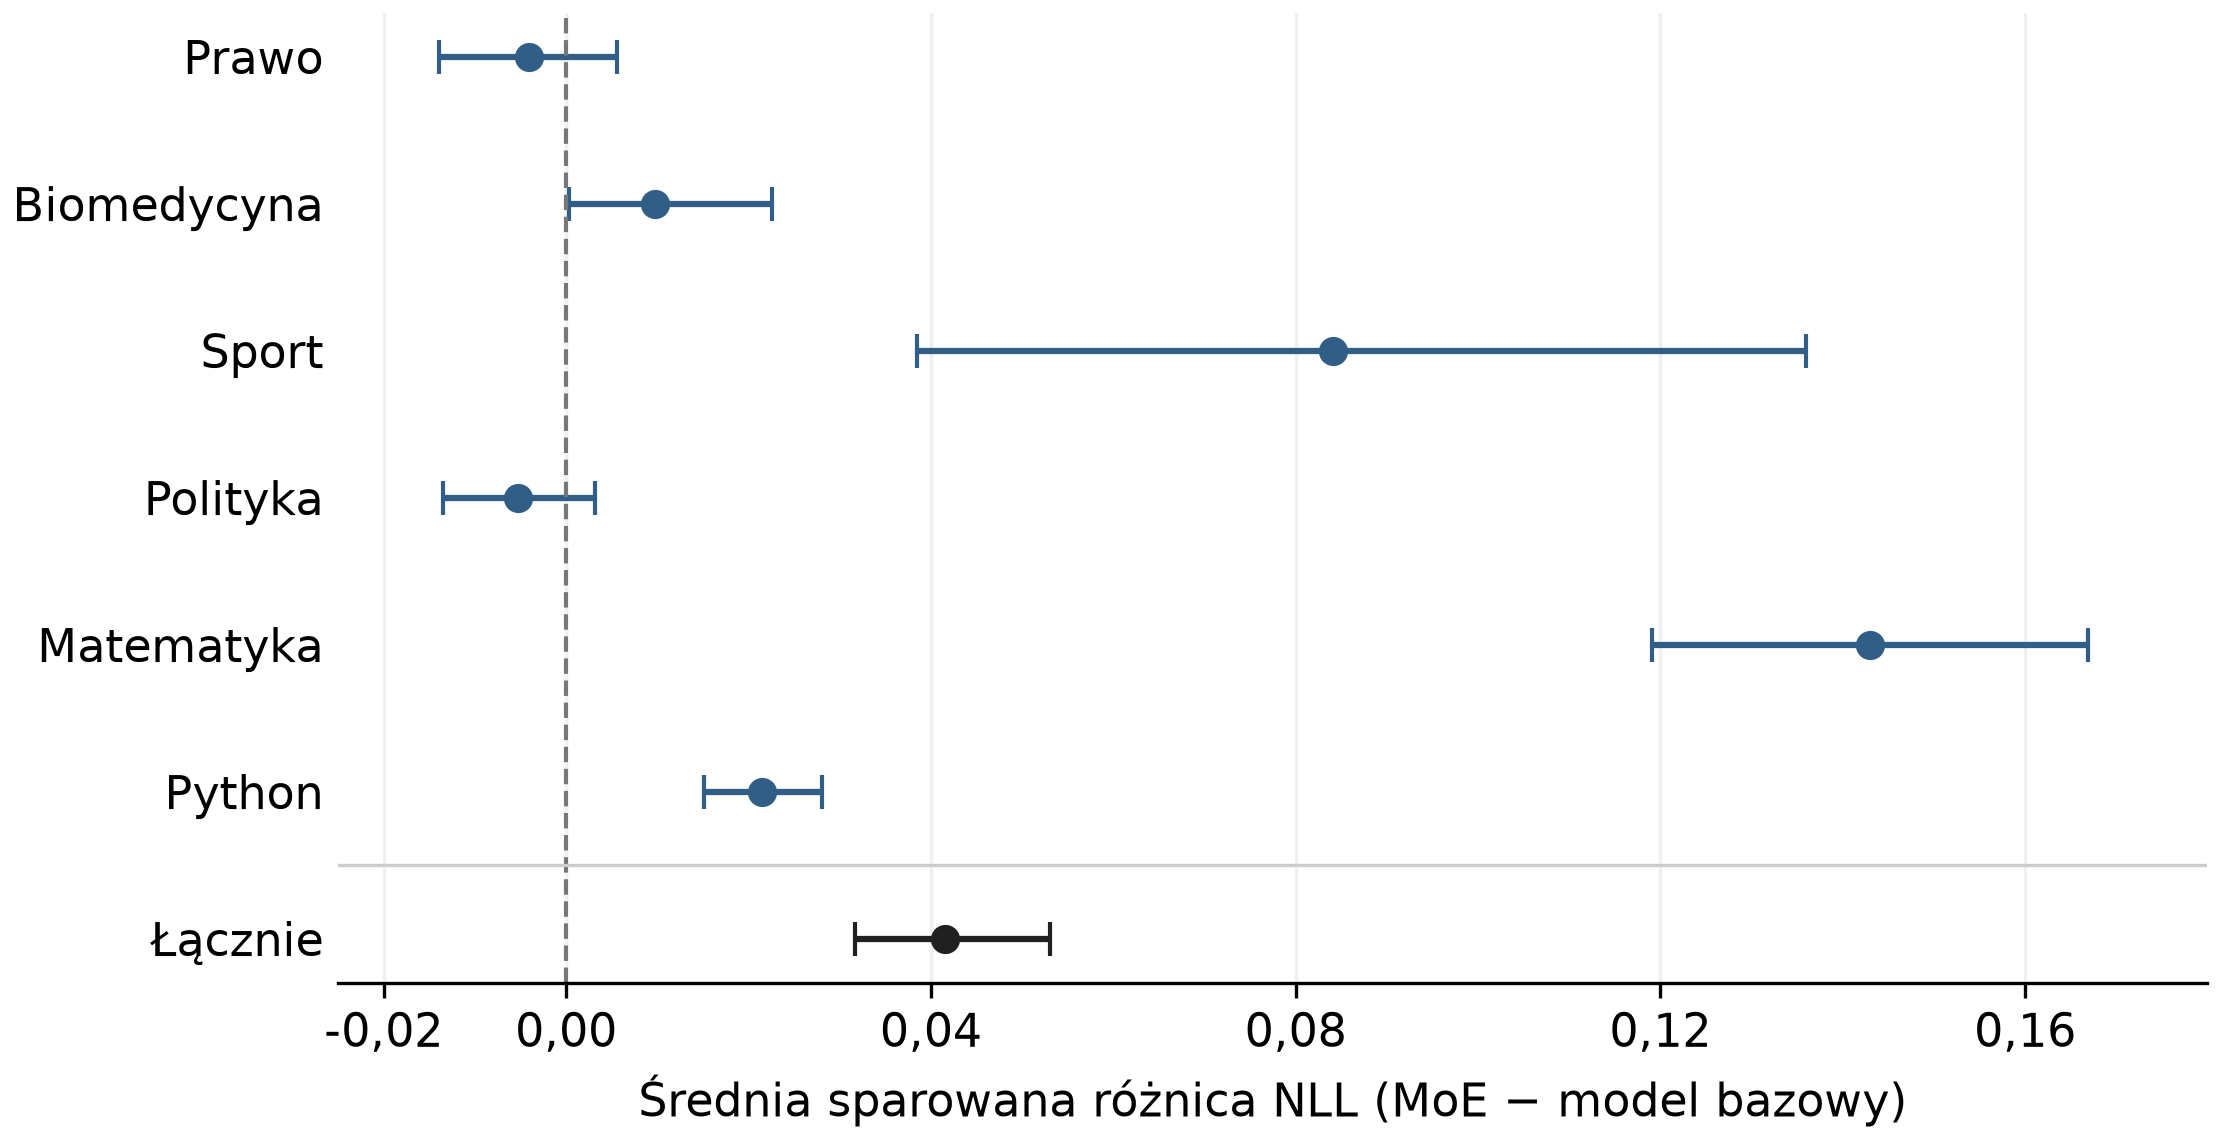
\includegraphics[width=\textwidth]{images/moe_validation_nll.png}
\caption{Średnie sparowane różnice NLL odpowiedzi referencyjnych wraz z przedziałami ufności $95\%$. Wartości dodatnie oznaczają pogorszenie MoE w benchmarku. Każda domena obejmuje $100$ przykładów, a wynik łączny -- $600$ przykładów o jednakowej wadze. Wykres opracowano na podstawie zapisanych wyników benchmarku.}
\label{fig:walidacja_nll}
\end{figure}

Przy nadaniu jednakowej wagi każdemu przykładowi wszystkie domeny mają taki sam udział w wyniku. Przy ważeniu liczbą tokenów odpowiedzi NLL wzrosło z $1{,}1818$ do $1{,}2277$, a PPL z $3{,}2603$ do $3{,}4135$, czyli o $4{,}70\%$. Tę agregację zdominował Python, obejmujący $6567$ spośród $7067$ tokenów odpowiedzi. Nie należy więc utożsamiać różnicy średnich ważonych tokenami ze średnią różnic dla przykładów przedstawioną na wykresie. \newline
Trafność odpowiedzi zmieniła się w znacznie mniejszym stopniu niż NLL (tabela~\ref{tab:walidacja_mc}). Łączna liczba trafień wzrosła ze $156$ do $158$ na $500$ pytań, czyli z $31{,}2\%$ do $31{,}6\%$. Przedział ufności dla zmiany wynosi $[-1{,}0;\,1{,}8]$ punktu procentowego. W polityce MoE poprawiło trzy odpowiedzi. Po uśrednieniu wyników dla różnych kolejności opcji trafność wzrosła z $30{,}67\%$ do $31{,}27\%$.

\begin{table}[htbp]
\centering
\begin{tabular}{lrrr}
\toprule
Domena & Model bazowy & MoE & Zmiana [p.p.] \\
\midrule
Prawo & $21\%$ & $20\%$ & $-1$ \\
Biomedycyna & $29\%$ & $29\%$ & $0$ \\
Sport & $50\%$ & $50\%$ & $0$ \\
Polityka & $35\%$ & $38\%$ & $+3$ \\
Matematyka & $21\%$ & $21\%$ & $0$ \\
\bottomrule
\end{tabular}
\caption{Trafność odpowiedzi modelu bazowego i MoE przy pierwotnej kolejności opcji, po $100$ pytań na domenę. Sport ma dwie opcje odpowiedzi, a pozostałe domeny po cztery.}
\label{tab:walidacja_mc}
\end{table}

Analiza kolejności odpowiedzi ujawniła to samo ograniczenie co w ocenie samodzielnych ekspertów. W sporcie baza i MoE wybierały A we wszystkich $200$ ocenach, a w matematyce we wszystkich $300$. Uzyskana trafność nie potwierdza zatem rozumienia zdań sportowych ani wykonywania działań arytmetycznych. Duży wzrost NLL oznacza mniejsze prawdopodobieństwo poprawnych etykiet, ale nie utratę wcześniej wykazanej umiejętności rozwiązywania tych zadań. W prawie, biomedycynie i polityce zgodność treści wybieranej odpowiedzi między kolejnościami opcji wynosiła jedynie około $55$--$57\%$, co również ogranicza interpretację trafności jako miary wiedzy. \newline
W generacji Pythona parsowalność kodu wyniosła $96\%$ dla bazy i $94\%$ dla MoE. W parach wystąpiły trzy poprawy i pięć pogorszeń, z $p\approx0{,}727$, więc wynik nie rozstrzyga o zmianie jakości składni. \newline
Na wspólnych zadaniach MoE uzyskało niższe średnie NLL niż właściwy samodzielny ekspert w pięciu domenach; wyjątkiem był sport. W Pythonie parsowalność wyniosła odpowiednio $94\%$ i $74\%$. Warunkowe użycie ekspertów ogranicza więc część pogorszeń obserwowanych przy stosowaniu przyciętego MLP do wszystkich tokenów. Nie dowodzi to przewagi samego routera: MoE korzysta również z nieprzyciętego MLP, a oba te elementy wpływają na wynik.


\section{Koszt obliczeń, generalizacja routera i ograniczenia wniosków}
\label{sec:generalizacja_routera}
\subsection{Koszt obliczeń modeli dziedzinowych}
\label{subsec:koszt_ekspertow}
Brak routera i fallbacku oznacza, że ekspert stale wykorzystuje $75\%$ szerokości badanego MLP. Redukuje to koszt projekcji tej warstwy o $25\%$, ale z racji na przeprowadzanie eksperymentu tylko na jednym bloku modelu, redukcja całkowita biorąc pod uwagę wszystkie warstwy MLP to jedynie około $1{,}389\%$. Liczba parametrów modelu z jednym ekspertem spada z $268\,098\,176$ do $267\,115\,136$, czyli o $0{,}367\%$. Zmierzona bazowa alokacja CUDA była niższa o $1{,}25$ MiB, natomiast zmiana szczytowej alokacji zależała od konfiguracji i nie zawsze była ujemna. 

\subsection{Koszt obliczeń i działanie routera w MoE}
\label{subsec:koszt_router_moe}
Telemetrię benchmarku MoE zbierano w osobnym przejściu przez same prompty, licząc każdy przykład jednokrotnie i pomijając padding. Nie obejmuje ona wielokrotnych ocen kandydatów w pytaniach wyboru ani kolejnych kroków generacji. Udziały routingu zestawiono w tabeli~\ref{tab:walidacja_routing}.

\begin{table}[htbp]
\centering
\small
\begin{tabular}{lrrr}
\toprule
Domena & Do ekspertów & Do zgodnego eksperta & Fallback \\
\midrule
Prawo & $22{,}10\%$ & $21{,}22\%$ & $77{,}90\%$ \\
Biomedycyna & $6{,}85\%$ & $4{,}76\%$ & $93{,}15\%$ \\
Sport & $24{,}53\%$ & $8{,}85\%$ & $75{,}47\%$ \\
Polityka & $3{,}65\%$ & $0{,}14\%$ & $96{,}35\%$ \\
Matematyka & $75{,}30\%$ & $75{,}30\%$ & $24{,}70\%$ \\
Python & $8{,}62\%$ & $0{,}11\%$ & $91{,}38\%$ \\
\bottomrule
\end{tabular}
\caption{Routing tokenów promptów w benchmarku MoE. Wszystkie odsetki są liczone względem ogółu tokenów danej domeny; kolumna zgodnego eksperta jest podzbiorem kolumny routingu do ekspertów.}
\label{tab:walidacja_routing}
\end{table}

Łącznie do ekspertów trafiło $19{,}64\%$ spośród $58\,246$ tokenów promptów, a pozostałe $80{,}36\%$ przetworzył bazowy MLP. Wśród skierowanych do ekspertów tokenów $84{,}79\%$ trafiło do eksperta zgodnego z domeną zadania, ale wynik ten jest zdominowany przez prawo i matematykę. W sporcie $616$ tokenów skierowano do matematyki, a tylko $348$ do sportu. W Pythonie były to odpowiednio $320$ tokenów skierowanych do matematyki i cztery do eksperta programistycznego. Do eksperta politycznego trafiło zaledwie $0{,}14\%$ tokenów zadań politycznych. Router może zatem częściowo rozpoznawać format tekstu zamiast jego dziedziny. Duży udział poprawnych skierowań w matematyce współistnieje z pogorszeniem NLL, więc sama zgodność eksperta z domeną nie gwarantuje jakości odpowiedzi. \newline
Duży udział sytuacji w której router nie wybierał eksperta tylko wracał do wariantu ogólnego ogranicza potencjalną oszczędność obliczeń. Korzystając z zależności wyprowadzonej w podrozdziale~\ref{sec:skladanie_moe}, otrzymano średnią efektywną szerokość zmodyfikowanego MLP równą $95{,}09\%$ szerokości bazowej. Dla trzech projekcji bramkowanego MLP koszt liniowy na token wynosi $C_{\mathrm{dense}}=3DH$, gdzie $D=640$ i $H=2048$. Po uwzględnieniu routera o sześciu wyjściach i udziału routingu $c$ przybliżony koszt ma postać:
\[
C_{\mathrm{MoE}}=(1-c)C_{\mathrm{dense}}+
0{,}75cC_{\mathrm{dense}}+6D.
\]
Przy zaobserwowanym routingu odpowiada to redukcji o około $4{,}81\%$ operacji mnożenia z akumulacją (ang. \textit{multiply--accumulate}, MAC) w MLP warstwy $9$. W odniesieniu do wszystkich $18$ modułów MLP jest to jedynie około $0{,}267\%$ ich łącznego kosztu liniowego. Udział w obliczeniach całego modelu jest jeszcze mniejszy, ponieważ pozostają mechanizmy uwagi i projekcja na słownik. \newline
Rachunek ten dotyczy rozkładu routingu zaobserwowanego na promptach, a nie zmierzonego kosztu pełnej generacji. Nie uwzględnia indeksowania tokenów, nieregularnych partii ekspertów ani transferów pamięci. Przechowywanie wag ekspertów obok bazowego MLP zwiększa zapotrzebowanie na pamięć; w badanej konfiguracji bazowa alokacja CUDA była większa o około $35{,}39$ MiB. Jest to konsekwencja zachowania pełnego MLP jako wariantu ogólnego, zgodnie z konstrukcją opisaną w rozdziale~\ref{chap:pruning_moe}. Architektura pozwala więc ograniczać liczbę operacji dla tokenów kierowanych do ekspertów, zachowując dostęp do nieprzyciętego modułu kosztem dodatkowej pamięci. \newline
Wyniki pokazują, że możliwe jest zbudowanie działającego MoE z ekspertów wyodrębnionych na podstawie domen semantycznych, przy zachowaniu trafności odpowiedzi i parsowalności kodu na poziomie zbliżonym do modelu bazowego. Ma to znaczenie w kontekście celu eksperymentu, ponieważ każdy wybrany ekspert wykorzystuje MLP o szerokości zmniejszonej o $25\%$. Usunięcie części neuronów może pogarszać jakość przewidywania, dlatego ograniczenie skali tego pogorszenia przy mniejszej liczbie operacji stanowi korzystny rezultat. \newline
W benchmarku zadań domenowych PPL MoE ważone liczbą tokenów wzrosło o $4{,}70\%$, a zmiany trafności odpowiedzi i parsowalności kodu były niewielkie i statystycznie nierozstrzygające. Wyniki wskazują zatem na zachowanie znacznej części jakości mierzonej tymi wskaźnikami. Nie oznacza to jednak jednakowo małego pogorszenia w każdej domenie: wzrost NLL był większy w sporcie i matematyce, a zależność wyboru odpowiedzi od jej pozycji ogranicza ocenę rzeczywistych umiejętności modelu. MoE uzyskało niższe średnie NLL niż samodzielni eksperci w pięciu z sześciu domen, co wskazuje na korzyść z warunkowego stosowania przyciętych modułów wraz z zachowaniem bazowego MLP. \newline
Mniejsza liczba mnożeń daje możliwość przyspieszenia obliczeń, ale jej wykorzystanie zależy od organizacji danych, rozdzielania tokenów między ekspertów i efektywności mnożenia macierzy na GPU. Optymalizacja tych elementów wykracza poza zakres pracy. Przedstawiona analiza określa zatem teoretyczną redukcję liczby operacji, bez utożsamiania jej z przyspieszeniem całego modelu.
